\chapter{Introduction and theory}
\label{chap:theory}

\section{The standard model of particle physics}
\label{sec:theory_sm}

\section{Standard model Higgs boson measurements}
\label{sec:theory_smH}

\section{Beyond the standard model}
\label{sec:theory_BSM}

\subsection{The Higgs sector of the MSSM}
\label{sec:theory_MSSM_H}

\subsection{\acl{2HDM}s}
\label{sec:theory_2HDM}

\section{MSSM benchmark scenarios}
\label{sec:theory_BSM_models}

\subsection{The $m_{h}^{\text{mod+}}$ scenario}
\label{sec:theory_BSM_models_mhmodp}

\subsection{MSSM scenarios at low \tanb}
A large area of the \mA-\tanb~plane in the $m_{h}^{\text{mod+}}$ 
scenario contains a light Higgs boson with a mass compatible with
125 GeV. However, at low values of \tanb this is not the case, with
values of \mh~dropping below 122 GeV. The low \tanb~regime can be re-opened
if $M_{\text{SUSY}}$ is allowed to be greater than 3 TeV \cite{MSSM-reopen}. 
MORE ABOUT FINE-TUNING
%But not too large, see ref above!
Figure \ref{fig:tanb_accessibility} shows contours of constant
light Higgs boson mass as a function of \tanb~and $M_{\text{SUSY}}$.
It indicates that values of \mh~can be compatible with 125$\pm$3 GeV
for \tanb~values down to 1 if $M_{\text{SUSY}}$ is around 100-1000 TeV. 
\tanb~values of 3-5 are even accessible for $M_{\text{SUSY}}$ of around 10 TeV.

\begin{figure}[h!]
\begin{center}
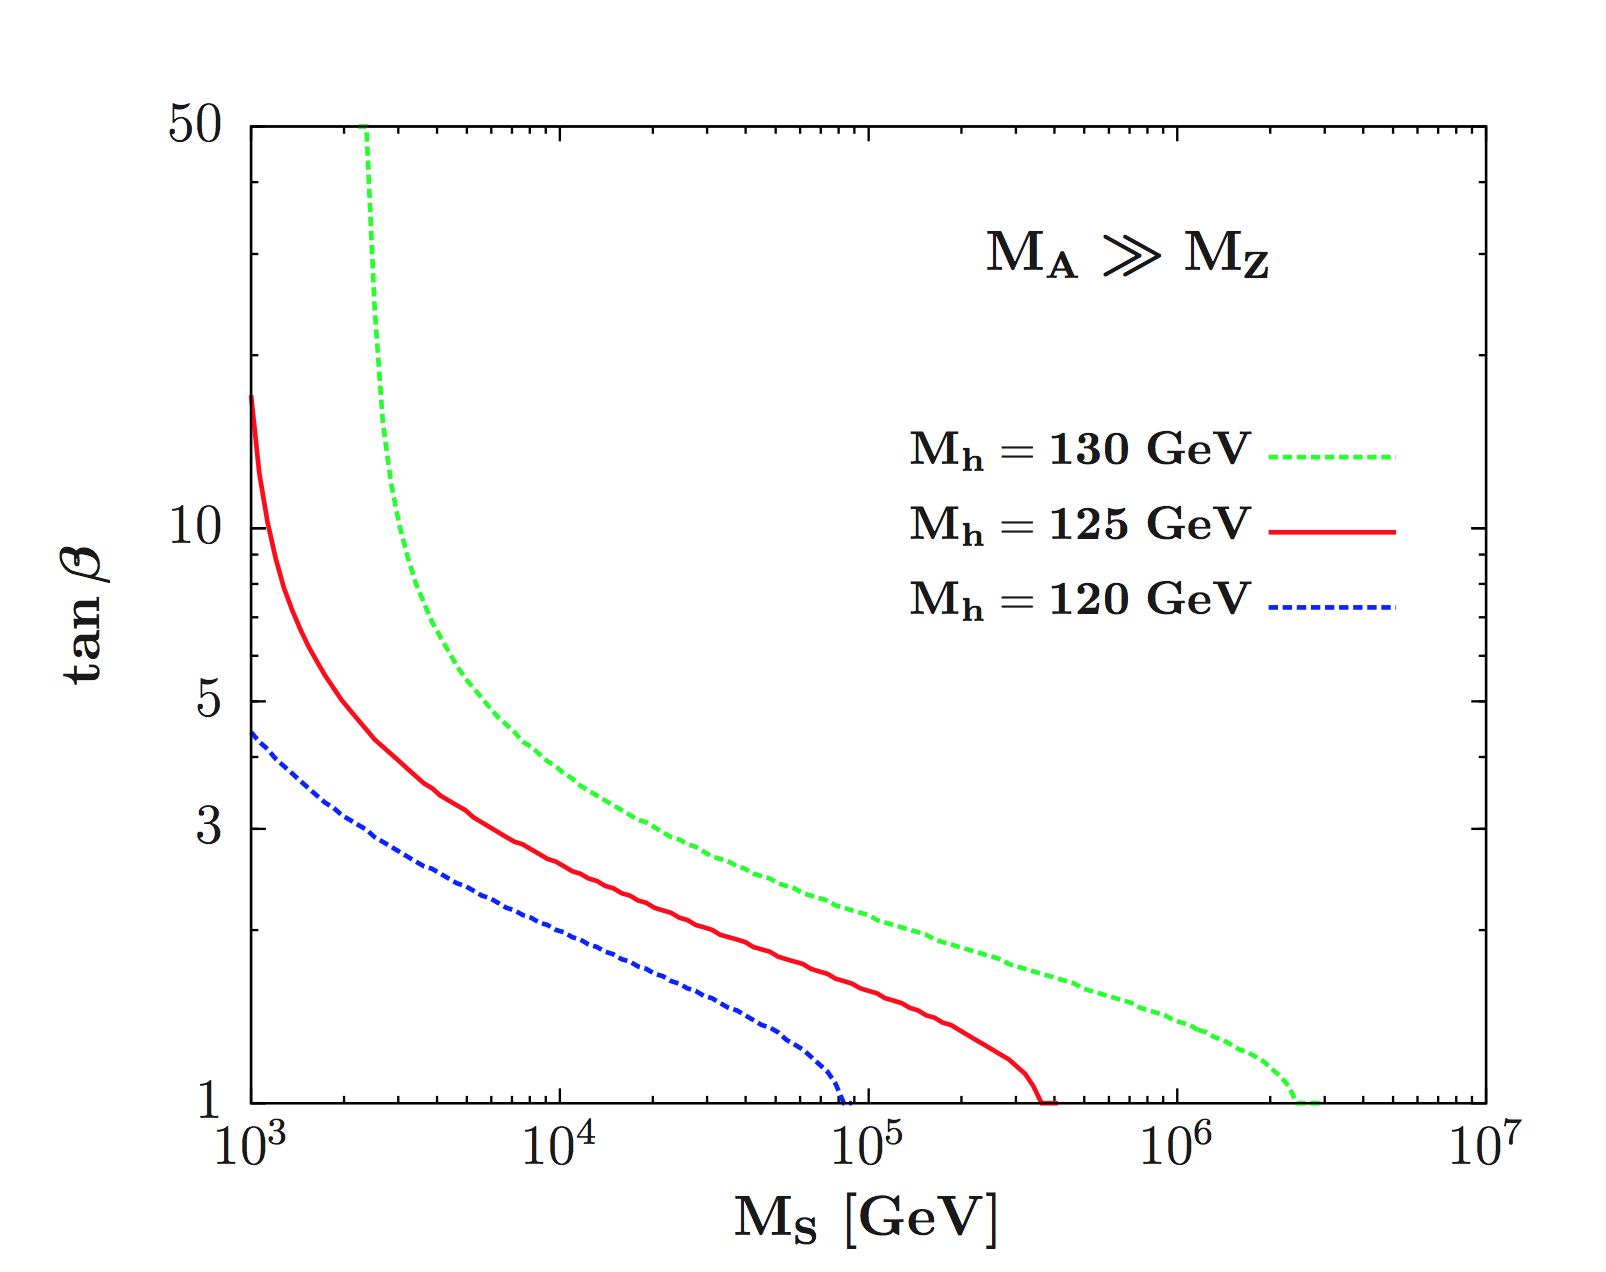
\includegraphics[width=0.5\textwidth]{./Theory/Figures/tanb_accessibility.png}
\end{center}
\caption{Contours of constant light Higgs boson mass as a function of \tanb~and $M_{\text{SUSY}}$.
High values of $M_{\text{SUSY}}$ allow for light Higgs boson masses compatible with
125 GeV down to low values of \tanb~\cite{hMSSM-2}.}
\label{fig:tanb_accessibility}
\end{figure}

%where the ±3 GeV variation corresponds to a rough estimate of the theoretical uncertainty of the MSSM prediction for mh, due to the unknown effect of higher-order correction

Gluon fusion dominance? Show decays? Or do it in the relevant subsecs?

Two approches for the definition of an MSSM scenario that gives
access to the low-\tanb~region have been developed, they will be
discussed in the next sections.

\subsubsection{The low-\tanb-scenario}
\label{sec:theory_BSM_model_lowtb}
In the low-\tanb-scenario \cite{Hein-low-tb-high,MSSM-lowtanb}, the SUSY parameters entering
the radiative corrections are tuned to obtain light 
Higgs boson masses of around 125 GeV in most of the \mA-\tanb~plane considered.
Figure \ref{fig:lowtbhigh_mh} shows that, apart from in a corner of \tanb~1-4 and 
\mA~150-250 GeV, \mh~is compatible with 125 GeV.

\begin{figure}[h!]
\begin{center}
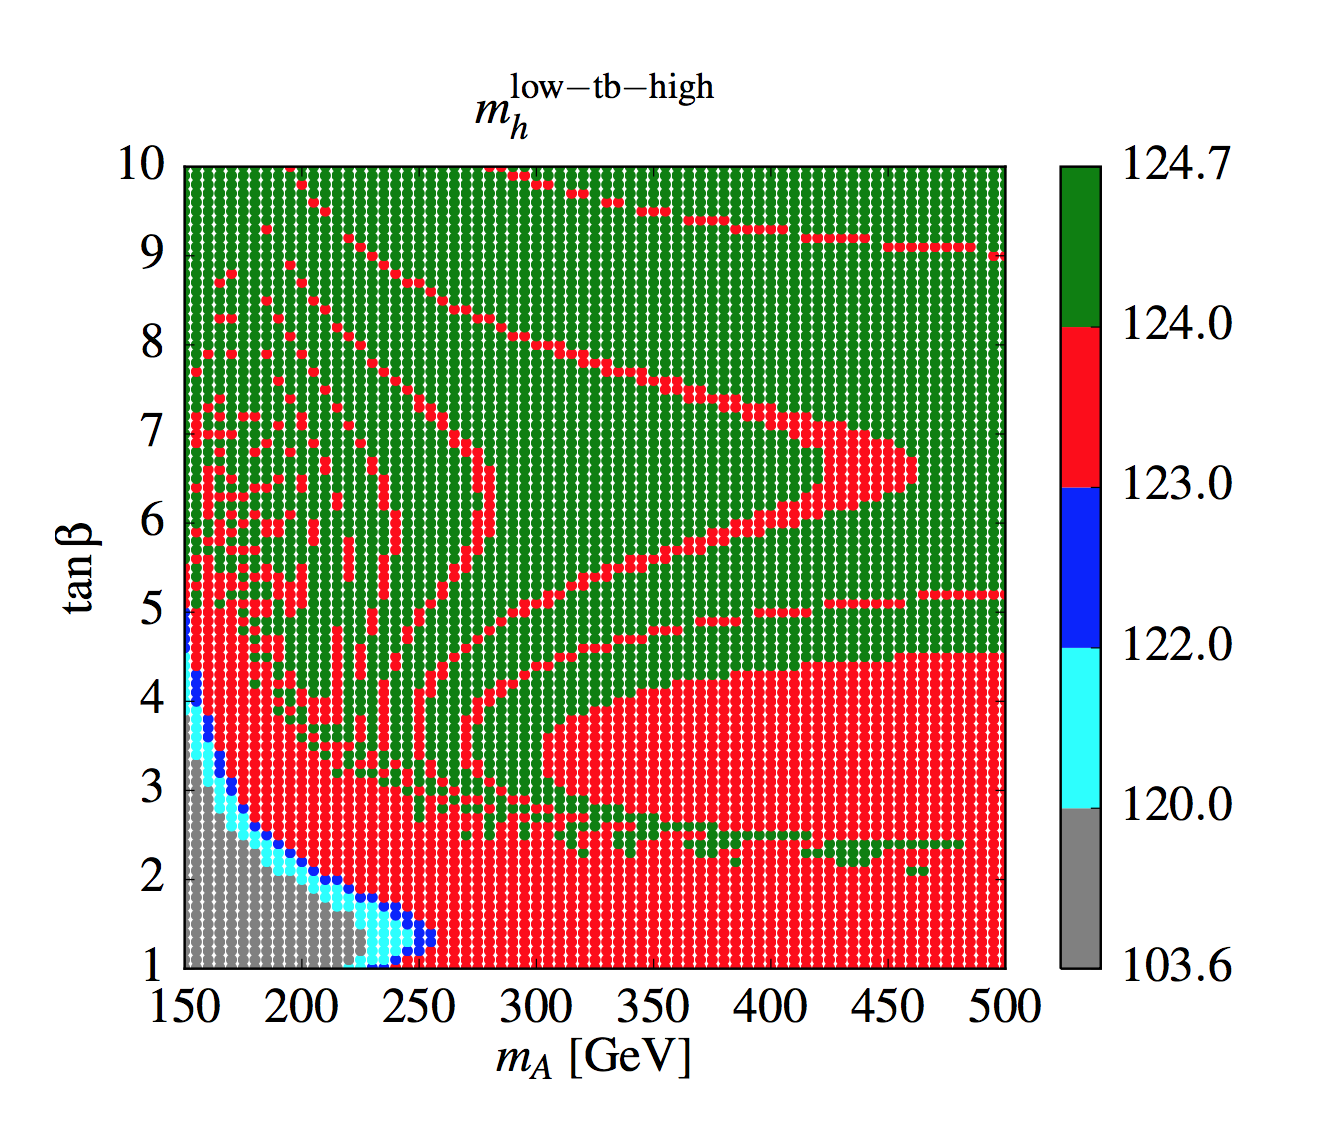
\includegraphics[width=0.5\textwidth]{./Theory/Figures/mh_lowtbhigh.png}
\end{center}
\caption{Mass of the light Higgs boson in the \mA-\tanb~plane of the low-\tanb~scenario.
The mass is compatible with 125 GeV nearly everywhere \cite{MSSM-lowtanb}.}
\label{fig:lowtbhigh_mh}
\end{figure}

To obtain \mh$\approx$125 GeV over a large part of the parameter
space, the SUSY parameters are chosen such that SUSY BREAKING MASSES ETC?
and $M_{\text{SUSY}}$ is not fixed but varies between a few TeV and 100 TeV, while
varying the parameter $X_t$ as:
\begin{equation}
\begin{split}
\tan{\beta} \leq 2 &: \frac{X_t}{M_{\text{SUSY}}} = 2\\
2 < \tan{\beta} \leq 8.6 &: \frac{X_t}{M_{\text{SUSY}}} = 0.0375\text{tan}^2\beta - 0.7\tan{\beta} + 3.25\\
8.6 < \tan{\beta} &: \frac{X_t}{M_{\text{SUSY}}} = 0.
\end{split}
\end{equation}
The other trilinear couplings are set to 2 TeV, with $\mu$ set to 1.5 TeV and $M_2$ to 2 TeV.

The branching fractions of \Htohh and \AtoZh in the low-\tanb~scenario are shown in
figure \ref{fig:lowtbhigh_br}. For both decay channels there are areas in the \mA-\tanb~plane
where the branching ratio is enhanced, indicating how analyses targeting such processes 
can be sensitive in this scenario. %REPHRASE
The analysis presented in chapter \ref{chap:hhh} is interpreted
in the low-\tanb~scenario.

\begin{figure}[h!]
\begin{center}
\subfloat[\Htohh]{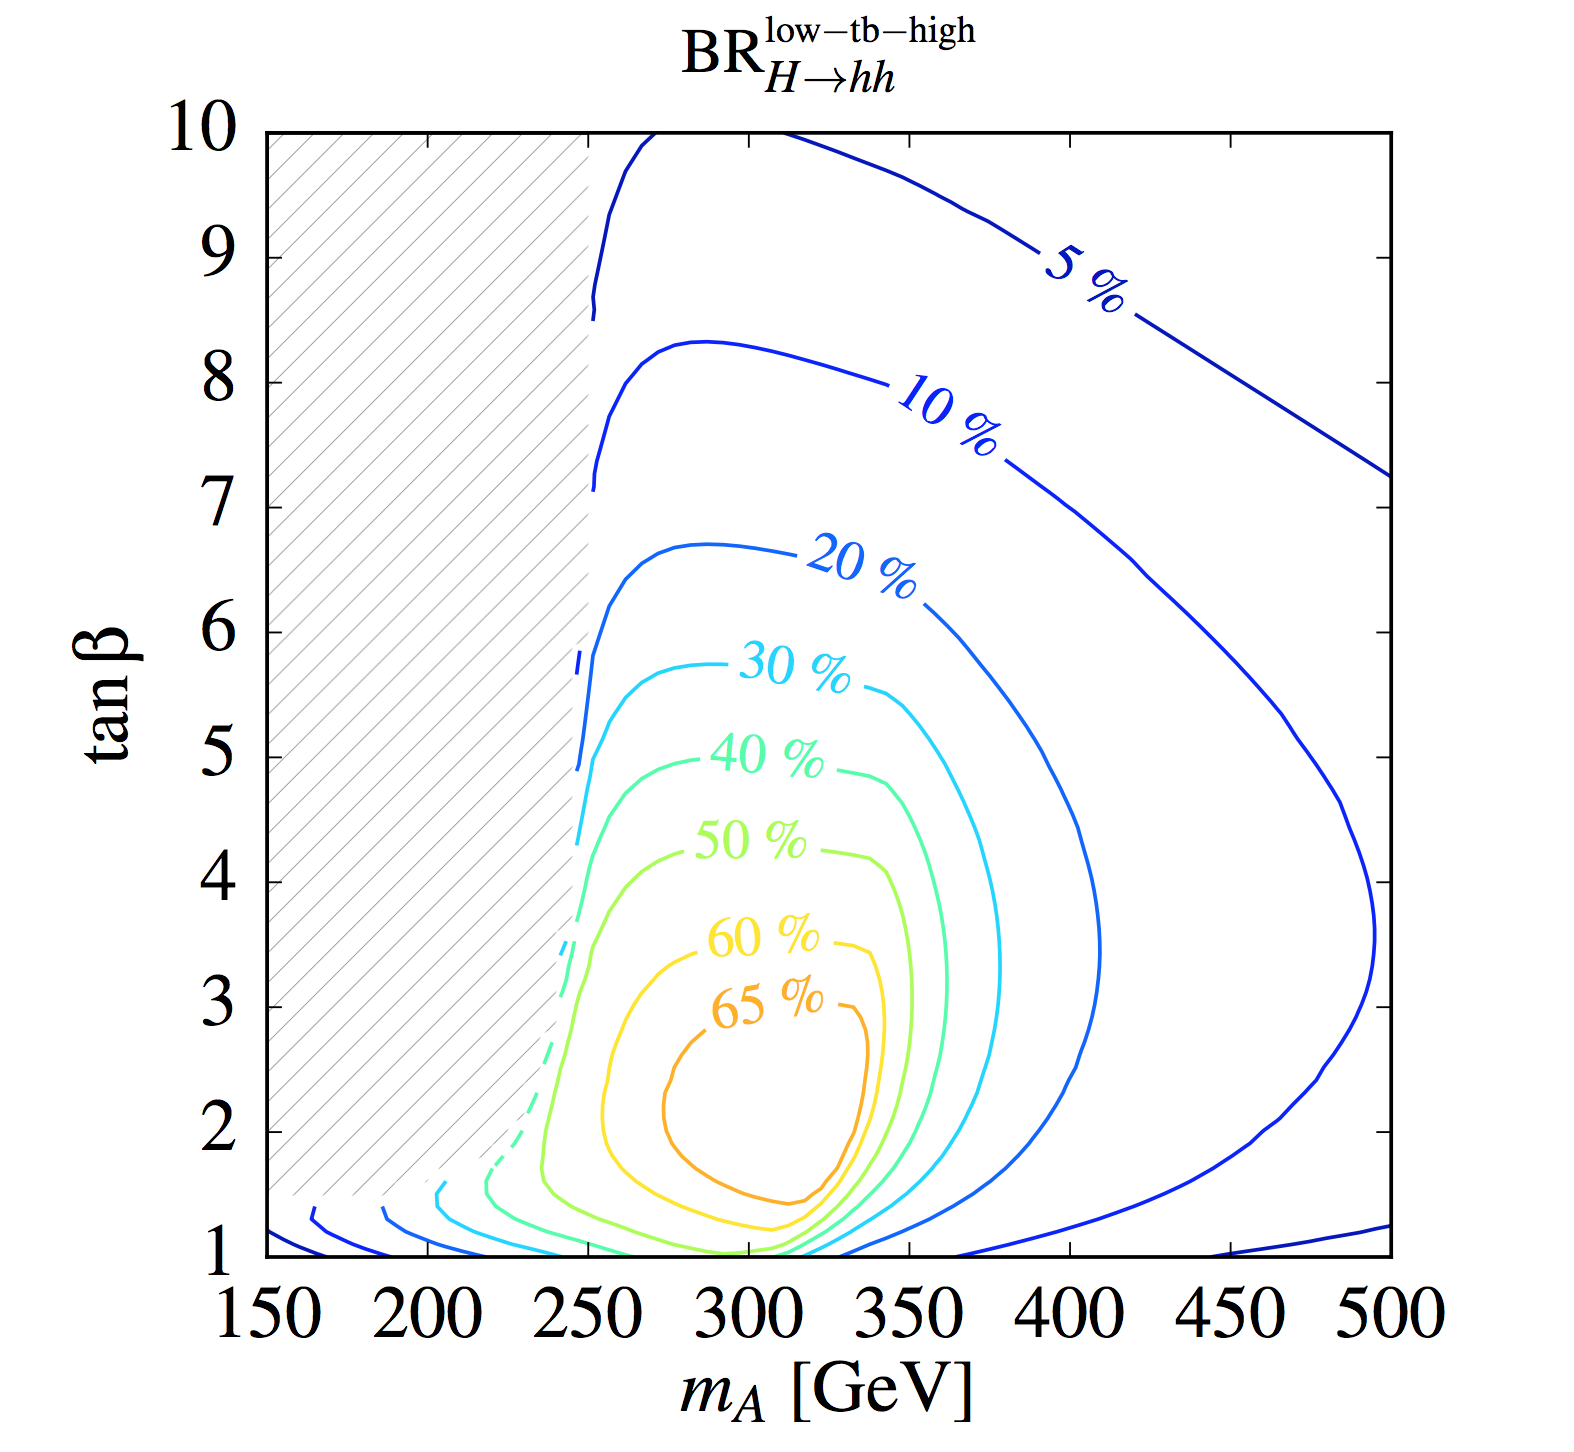
\includegraphics[width=0.5\textwidth]{./Theory/Figures/lowtbhigh_hhbr.png}}
\subfloat[\AtoZh]{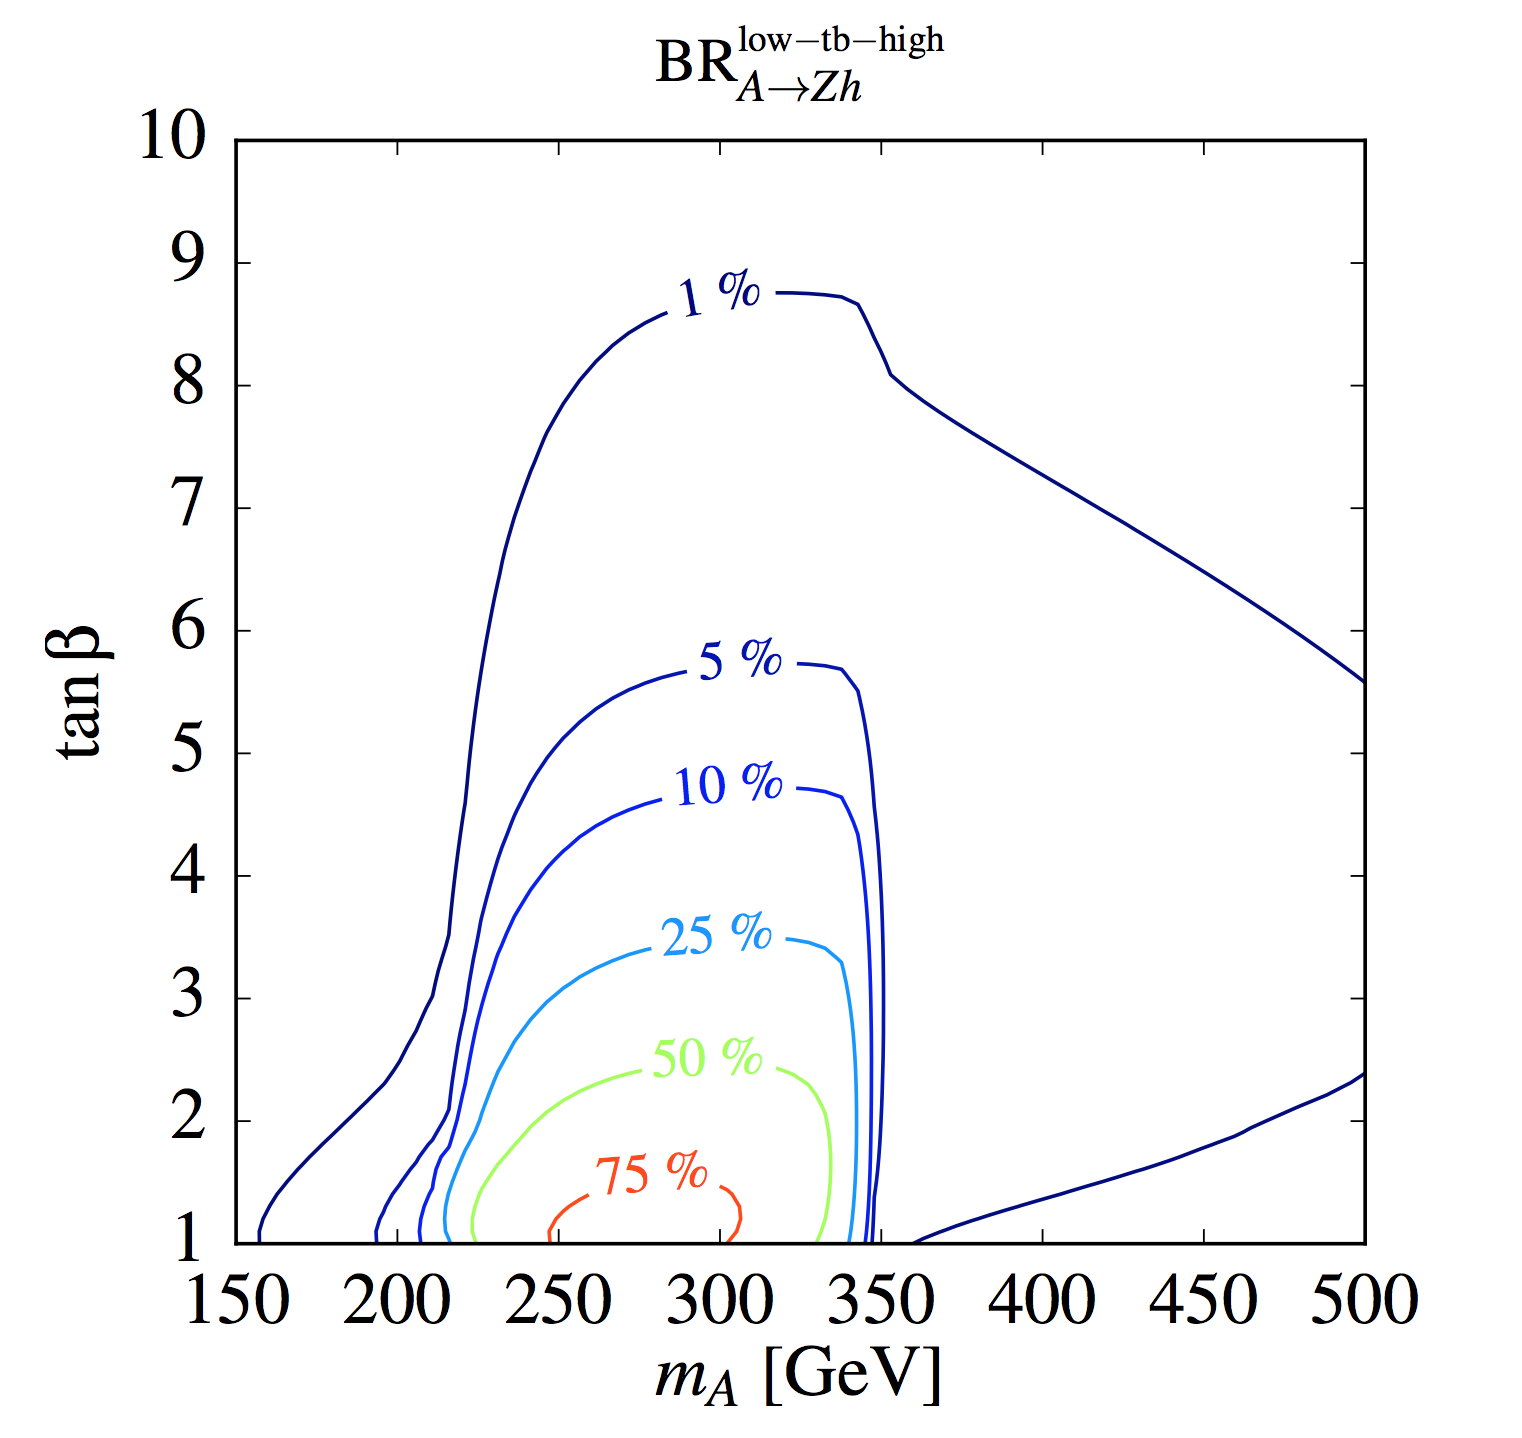
\includegraphics[width=0.5\textwidth]{./Theory/Figures/lowtbhigh_azhbr.png}}
\end{center}
\caption{Branching fractions of (a) \Htohh and (b) \AtoZh in the low-\tanb~scenario, indicating 
areas where both are significantly enhanced \cite{MSSM-lowtanb}.}
\label{fig:lowtbhigh_br}.
\end{figure}

\subsubsection{The hMSSM scenario}
\label{sec:theory_BSM_models_hMSSM}
The hMSSM scenario \cite{hMSSM-1,hMSSM-2} uses a different approach by starting from 
the REPHRASE tree-level expressions for masses and mixing and
the mass of the light Higgs boson \mh=125 GeV.

One of the assumptions of the hMSSM is that the
the mass matrix for the neutral CP-even states can
be decomposed as,
\begin{equation}
\label{eqn:hmssm_massmatrix}
\mathcal{M}^2_{\phi} = \mathcal{M}^2_{\text{tree}} + \begin{pmatrix}
\Delta\mathcal{M}^2_{11} & \Delta\mathcal{M}^2_{12} \\
\Delta\mathcal{M}^2_{12} & \Delta\mathcal{M}^2_{22} \end{pmatrix},
\end{equation}
where the $\Delta\mathcal{M}^2_{ij}$ are the radiative corrections.
The second assumption is that only $\Delta\mathcal{M}^2_{22}$ needs to be
taken into account, as this is the element that involves the stop-top correction
and so $\Delta\mathcal{M}^2_{22} >> \Delta\mathcal{M}^2_{12},\Delta\mathcal{M}^2_{11}$. 
Finally, all SUSY particles are assumed to be heavy enough not to be
detected at the \acs{LHC} and apart from effects on the mass matrix, 
the effects on the Higgs sector can be neglected.
%all SUSY particles are heavy enough to escape detection at the LHC, and their effects on the Higgs sector other than those on the mass matrix, e.g. via direct loop corrections to the Higgs-boson couplings or via modifications of the total decay widths, can be neglected.

Using these assumptions we can invert the lightest eigenvalue
of the mass matrix to get: 
\begin{equation}
\label{eqn:hmssm_deltam22}
\Delta\mathcal{M}^2_{22} = \frac{m_h^2(m_A^2+m_Z^2 - m_h^2) - m_A^2m_Z^2\text{cos}^22\beta}{m_Z^2\text{cos}^2\beta + m_A^2\text{sin}^2\beta - m_h^2},
\end{equation}

This means we can write,
\begin{equation}
\label{eqn:hmssm_mHalpha}
\begin{split}
&m^2_H = \frac{(m_A^2+m_Z^2-m_h^2)(m_z^2\cos{\beta}^2+m_A^2\sin{\beta}^2 - m_A^2m_Z^2\cos{2\beta}^2}{m_Z^2\cos{\beta}^2+m_A^2\sin{\beta}^2-m_h^2},\\
&\tan{\alpha} = -\frac{(m_Z^2+m_A^2)\cos{\beta}\sin{\beta}}{m_Z^2\cos{\beta}^2+m_A^2\sin{\beta}^2-m_h^2}.
\end{split}
\end{equation}
Combining this with the Hhh coupling,
\begin{equation}
\label{eqn:hmssm_Hhh}
\lambda_{Hhh} = \lambda_{Hhh,tree} + 3\frac{\Delta\mathcal{M}^2_{22}\sin{\alpha}}{m_Z^2\sin{\beta}}\cos{\alpha}^2,
\end{equation}
gives enough information to determine the cross sections and branching
ratios of all the five Higgs bosons as a function of \mA~and \tanb. The scenario
is only well defined in regions where the denominator in equations
\ref{eqn:hmssm_deltam22} and \ref{eqn:hmssm_mHalpha}, $m_Z^2\cos{\beta}^2+m_A^2\sin{\beta}^2 - m_h^2$, is nonzero. 
This leads to a minimum accesible \mA~value of \mh~at high \tanb, and
a minimum accessible \mA~of around 151 GeV for \tanb=1. In addition, the scenario
can be formulated, but is not strictly valid, for values of \tanb upwards of 10 \cite{CMS-PAS-HIG-16-007}.
The reason for this is that direct higher order SUSY corrections to down-type
fermion couplings and corrections due to SUSY particles in loops become relevant
above \tanb=10, but these are omitted in the hMSSM approach.

%to the couplings to the h, as expected from the SM, as will be further discussed in Section 3. This scenario is strictly valid for mA > 130 GeV and tanβ < 10. It can still be formulated for values up to tanβ < 60 though the omission of direct higher order SUSY corrections to down-type fermion couplings (also referred to as ∆β corrections) and corrections due to SUSY particles in loops, which be- come relevant for tan β > 10 question the consistency of the predictions with SUSY. A detailed

The production cross--sections at $\sqrt{s}=14$ TeV for gluon fusion production of the
H and A bosons, as well as for b-associated production, are shown in figure \ref{fig:hmssm_xs}.
As expected, gluon fusion production is dominant at low \tanb,with b-associated
production being more important at high \tanb. The cross sections increase for increasing \tanb,
apart from the gluon fusion cross section at low \tanb, where it decreases as \tanb~increases
due to a negative top-bottom intereference effect.

\begin{figure}[h!]
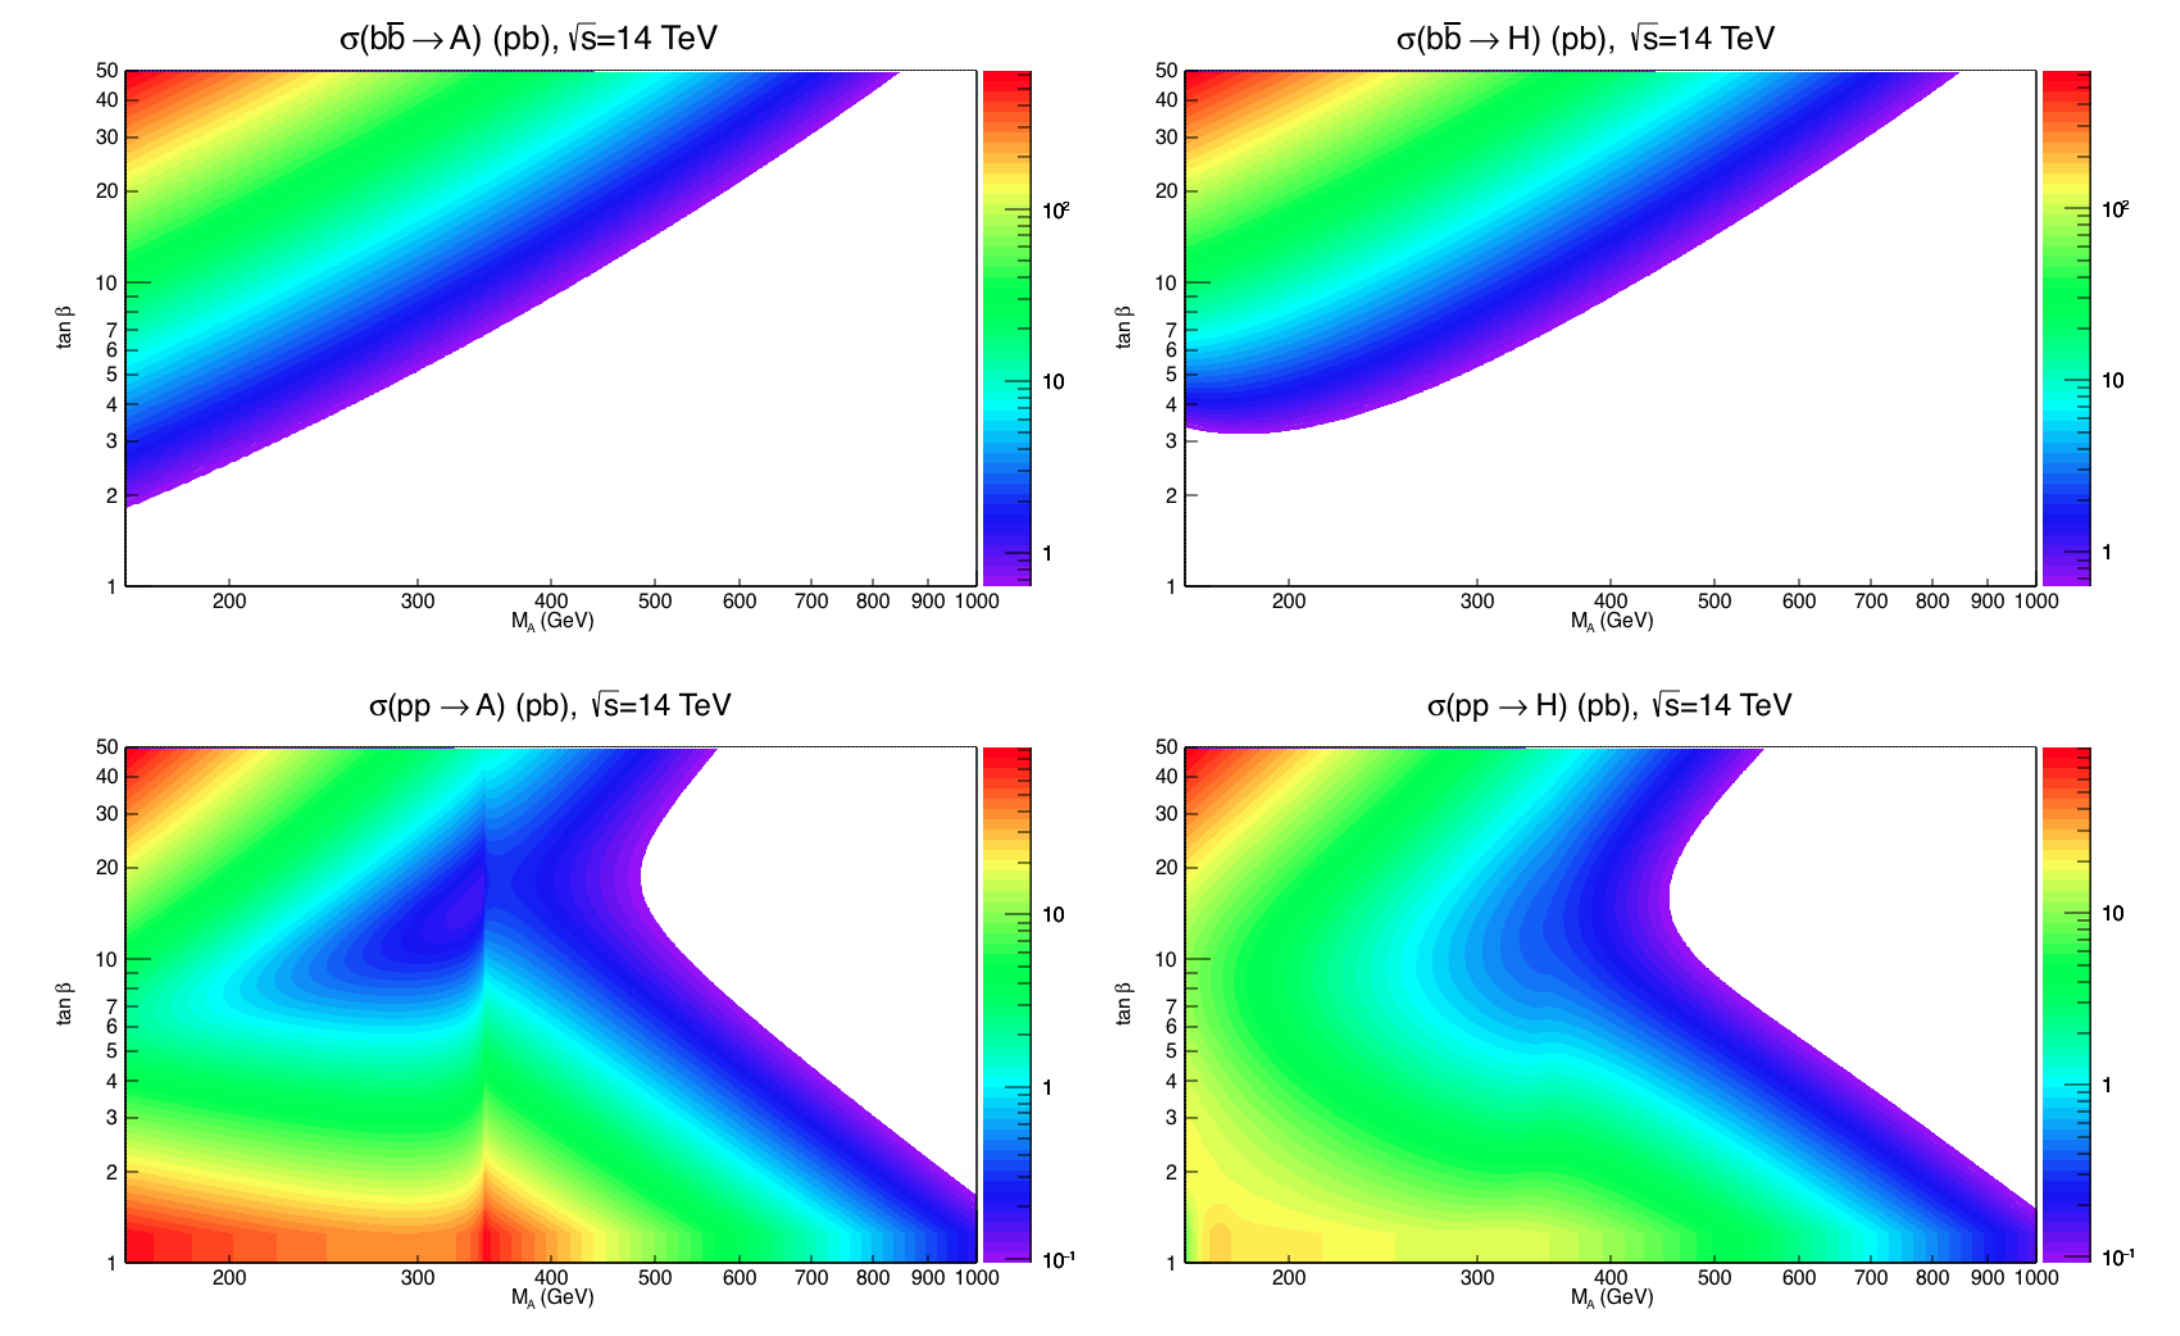
\includegraphics[width=\textwidth]{./Theory/Figures/hmssm_xsAH.png}
\caption{Cross-sections at $\sqrt{s}=14$ TeV as a function of
\mA~and \tanb~ in 
the hMSSM scenario for b-associated production of \PHiggsps (top left), b-associated
production of \PHiggs (top right), gluon fusion production of \PHiggsps (bottom left) and
gluon fusion production of \PHiggs (bottom right). The white areas indicate cross-sections
smaller than the minimum value on the z-axis. We can generally see the cross-sections increase
with growing \tanb, apart from the gluon fusion cross sections which decrease with increasing
\tanb~for low \tanb~\cite{hMSSM-2}.}
\label{fig:hmssm_xs}
\end{figure}

Figure \ref{fig:hmssm_brtautau} shows the branching ratios of \PHiggsps and \PHiggs into \Pgt\Pgt.
The branching ratios are large over a large part of the mA-\tanb~plane, but mostly so
at high \tanb.

\begin{figure}[h!]
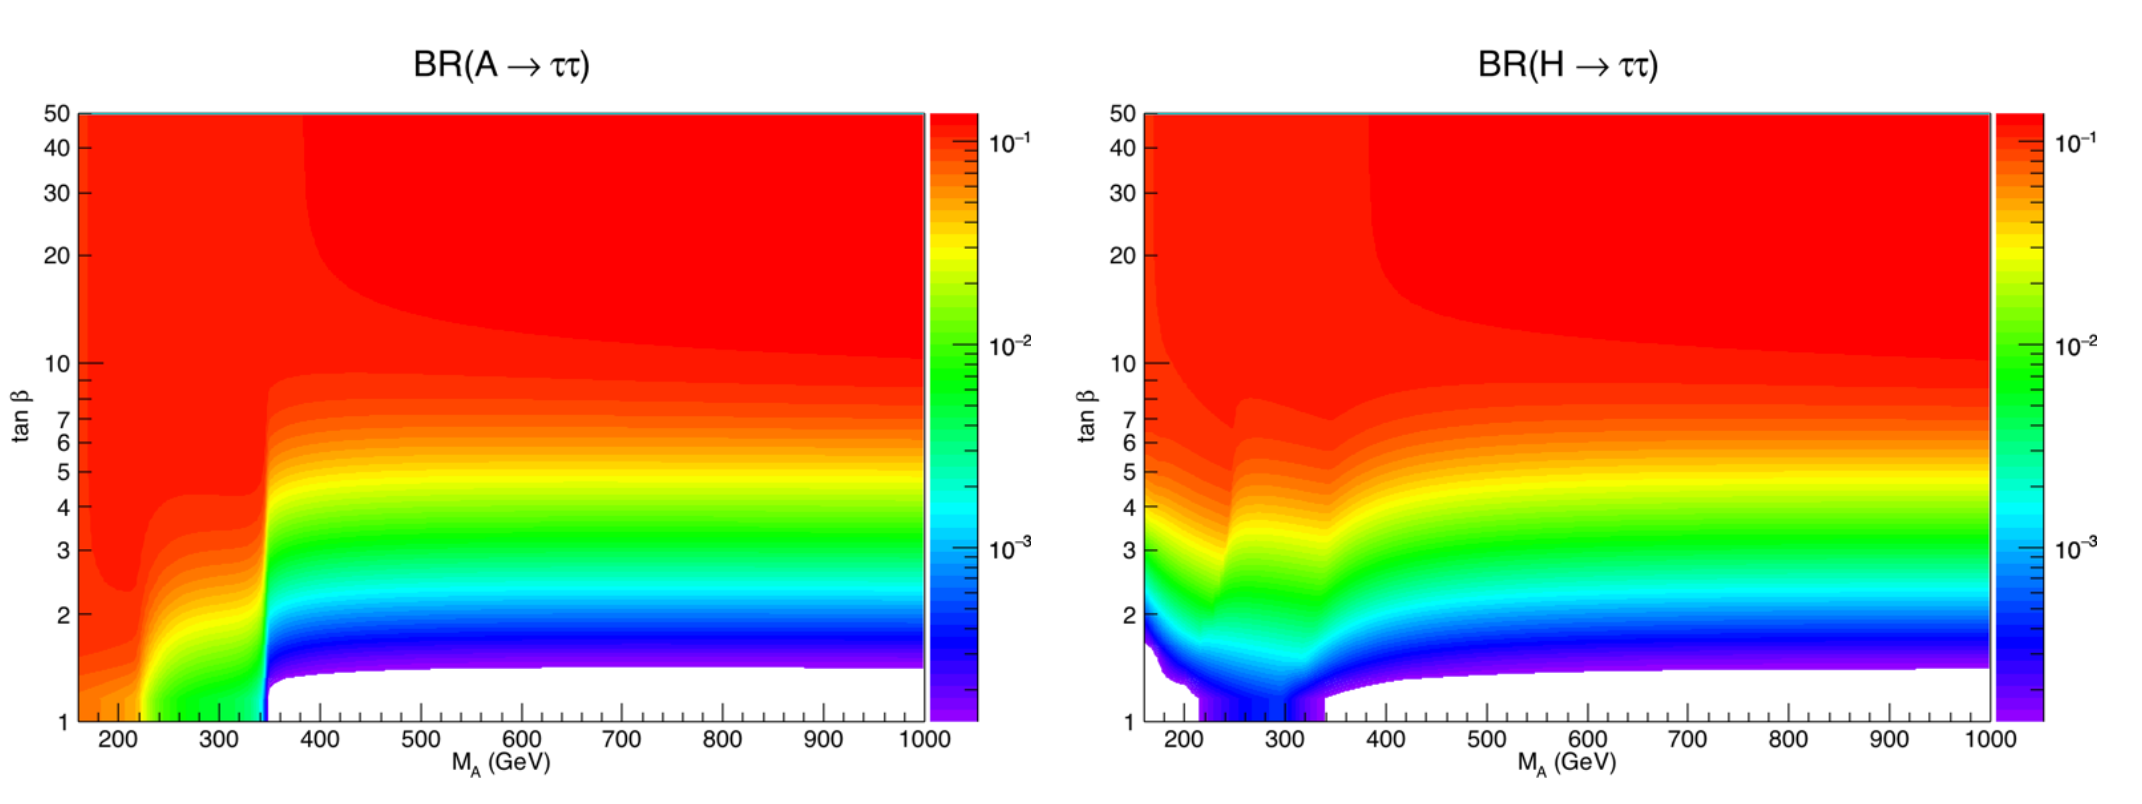
\includegraphics[width=\textwidth]{./Theory/Figures/hmssm_brtautau.png}
\caption{Branching ratios of \PHiggsps (left) and \PHiggs (right) into \tautau. The
branching ratio is enhanced at high \tanb~\cite{hMSSM-2}.} 
\label{fig:hmssm_brtautau}
\end{figure}


\section{Status of BSM Higgs boson searches}
\label{sec:theory_BSMH_status}
With the data collected during 
Run 1 of the \ac{LHC} many searches for BSM Higgs
bosons were already performed. The state of play with the full
Run-1 dataset collected by \ac{CMS} can be seen in figure \ref{fig:bsm_summary},
which shows the interpretations of different searches in the $m_{h}^{\text{mod+}}$ (figure \ref{fig:bsm_summary}a)
and hMSSM scenarios (figure \ref{fig:bsm_summary}b). The direct search for heavier Higgs bosons decaying into pairs
of tau leptons (shown in dark blue) sets the most stringent limits at high \tanb,with searches for 
heavy Higgs bosons decaying to $b\bar{b}$ and to $\mu\mu$ both excluding smaller parts of the high \tanb-region.
Searches for heavy Higgs bosons decaying to WW and ZZ are able to exclude part of the low-\tanb-region. In the 
hMSSM scenario searches for \Htohh and \AtoZh can exclude a small area at low \tanb~and between \mA=250-350 GeV.
The red exclusion contour in figure \ref{fig:bsm_summary}b is the re-interpretation of the analysis presented in
chapter \ref{chap:hhh}.

In Run-2 of the \ac{LHC} searches for \AHtotautau, setting more stringent limits than those shown in \ref{fig:bsm_summary},
have been performed in \ac{CMS}. The results of these searches will be presented in chapter \ref{chap:mssm}. Other searches
for heavy Higgs bosons with decays to other final states are also in progress as the Run-2 data keep
amassing. 

\begin{figure}[h!]
\begin{center}
\subfloat[$m_{h}^{\text{mod+}}$ scenario]{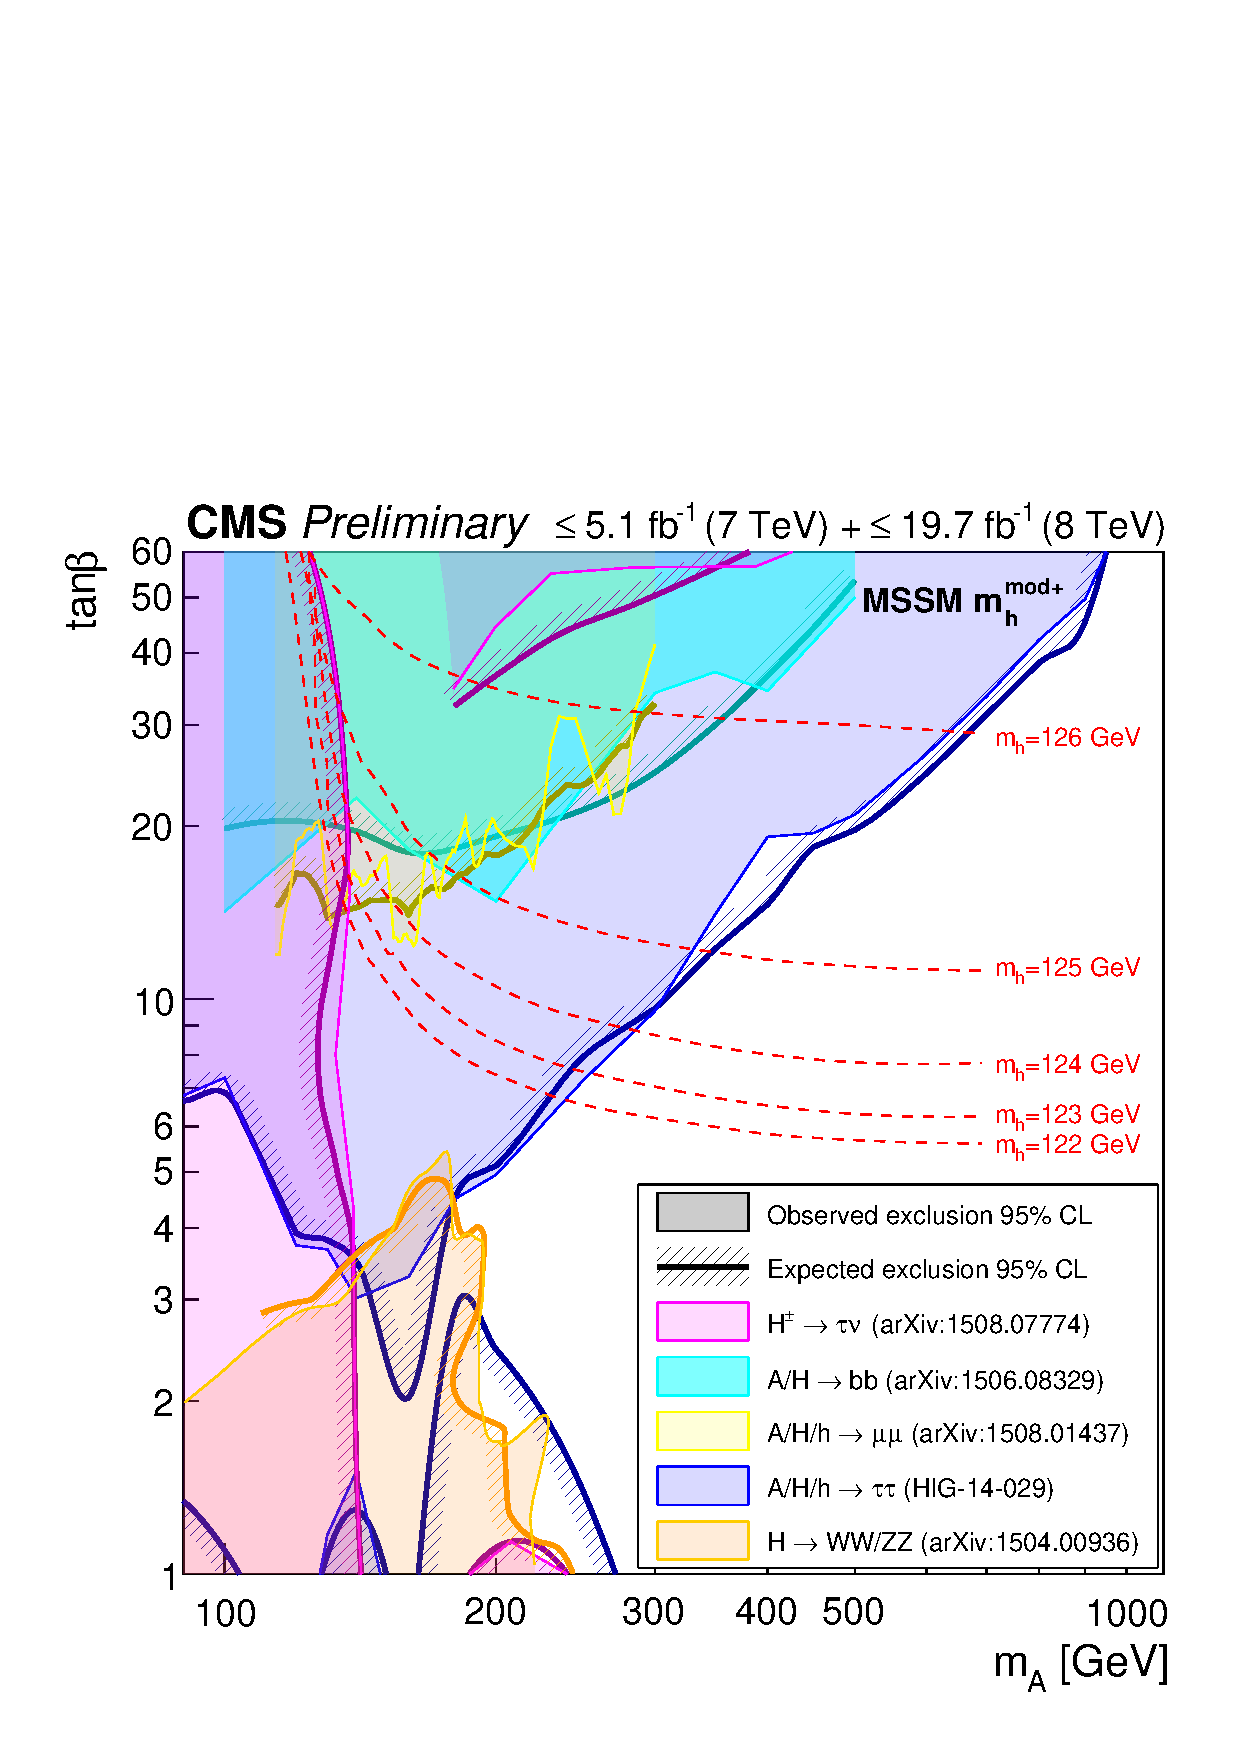
\includegraphics[width=0.5\textwidth]{./Theory/Figures/CMS-PAS-HIG-16-007_Figure_003-a.pdf}}
\subfloat[hMSSM scenario]{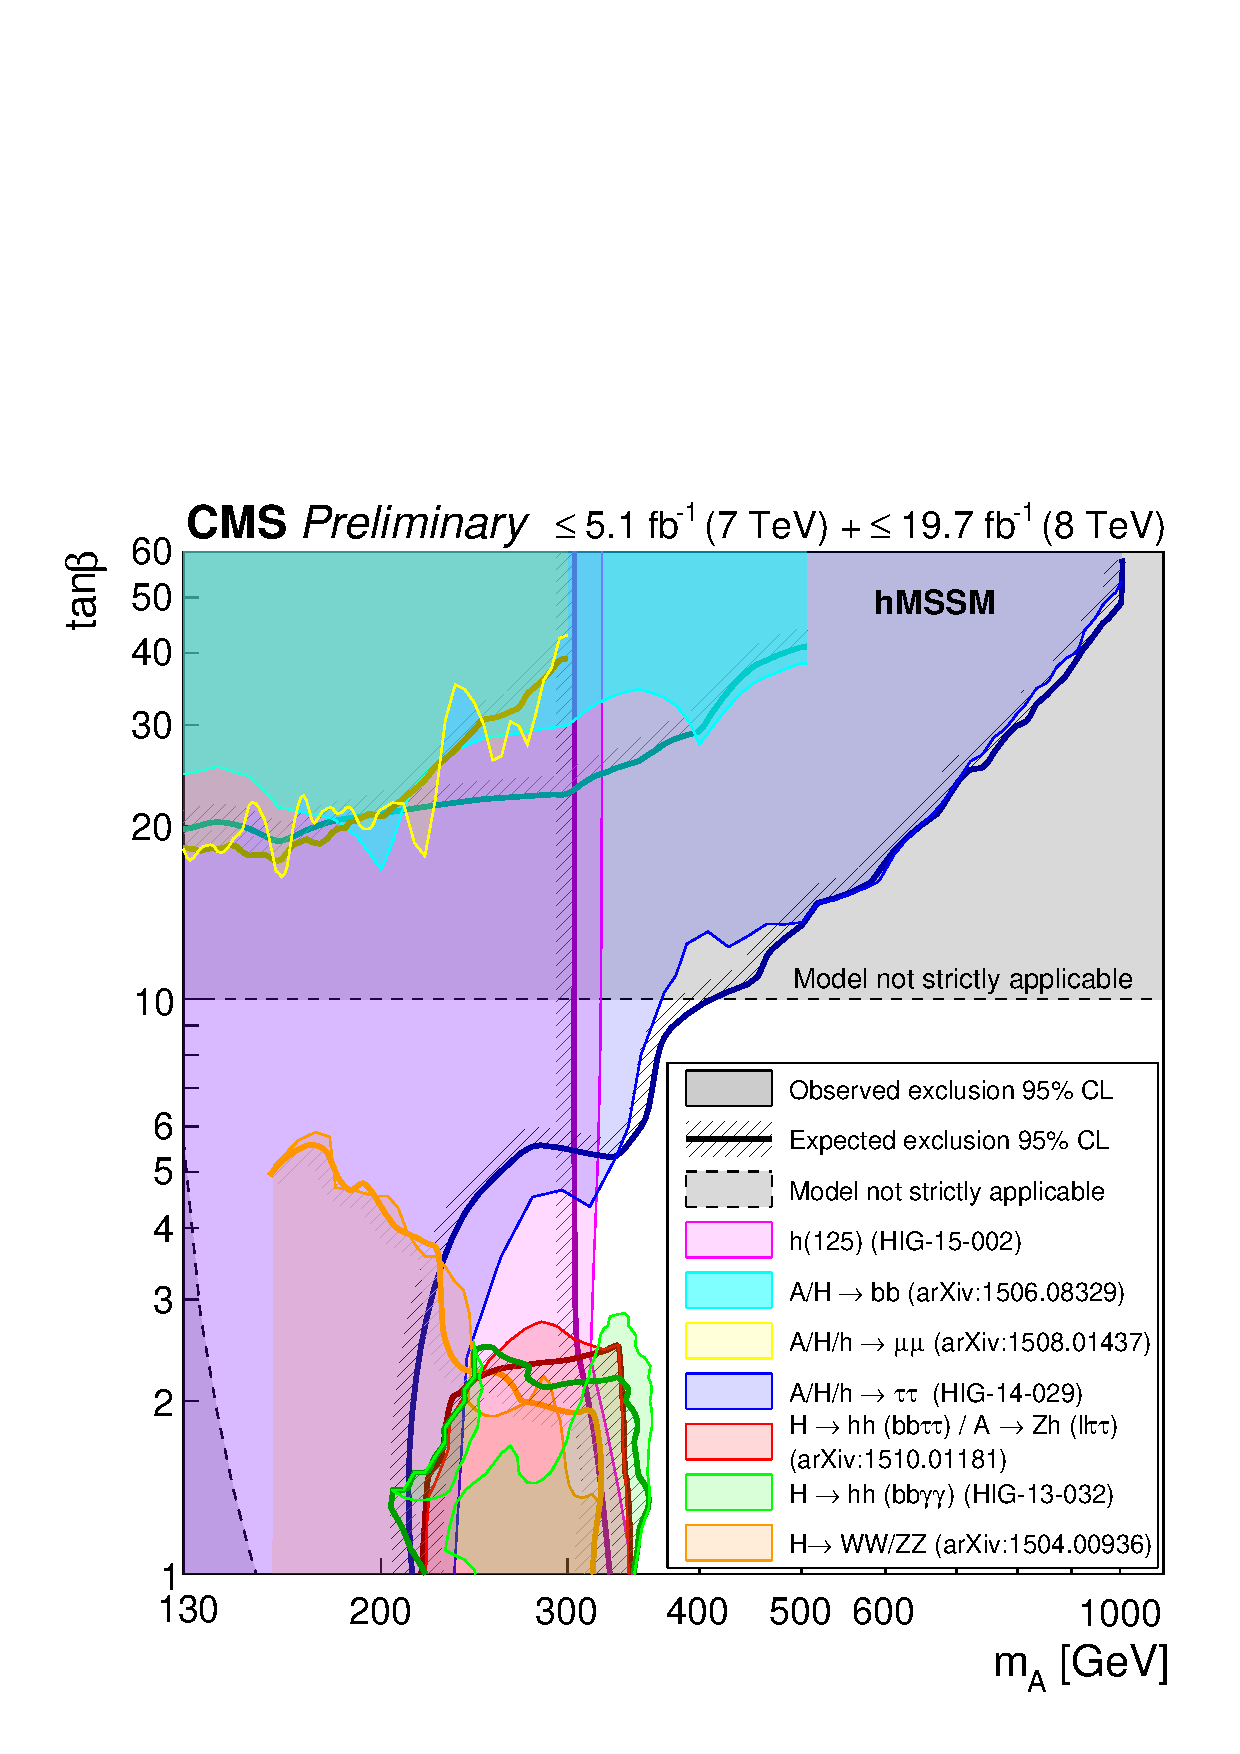
\includegraphics[width=0.5\textwidth]{./Theory/Figures/CMS-PAS-HIG-16-007_Figure_003-b.pdf}}
\end{center}
\caption{Summary of the interpretations of Run 1 BSM Higgs searches at \ac{CMS} in (a) the $m_{h}^{\text{mod+}}$ and (b) the
hMSSM scenario. The different coloured areas indicate the observed and expected exclusion from different searches in these
scenarios. The results from MSSM Higgs searches with decays into $\tau$ leptons are shown in blue and exclude more of the parameter
space than any of the other searches. The MSSM Higgs to $b\bar{b}$ (cyan) and Higgs to $\mu\mu$ (yellow) searches are also sensitive in part
of the high-\tanb region, with Higgs to WW or ZZ (orange) providing exclusion power at low \tanb~and low mass. In the $m_{h}^{\text{mod+}}$ 
scenario the charged Higgs to $\Pgt\Pgn$ search (magenta) excludes the low-mass region for all values of \tanb. Masses below around 300 GeV in the 
hMSSM scenario are excluded instead by constraints from standard model Higgs boson measurements (magenta). In this scenario small
areas of the low-\tanb~region are also excluded by the search for $H\rightarrow hh \rightarrow bb\tau\tau$ and $A\rightarrow Zh \rightarrow \ell\ell\tau\tau$ (red)
and the search for $H\rightarrow hh \rightarrow bb\gamma\gamma$ \cite{CMS-PAS-HIG-16-007}.}
\label{fig:bsm_summary}
\end{figure}


